\newcommand{\Quadrille}[1]{
\includegraphics[width=0.0#1\textwidth ]{icons/quadrille.png}}
\newcommand{\SCD}[1]{
\includegraphics[width=0.0#1\textwidth]{icons/scotlandcd.png}}
\newcommand{\CountryD}[1]{
\includegraphics[width=0.0#1\textwidth ]{icons/countrydance.png}}
\newcommand{\Waltz}[1]{
\includegraphics[width=0.0#1\textwidth]{icons/waltz.png}}
\newcommand{\Else}[1]{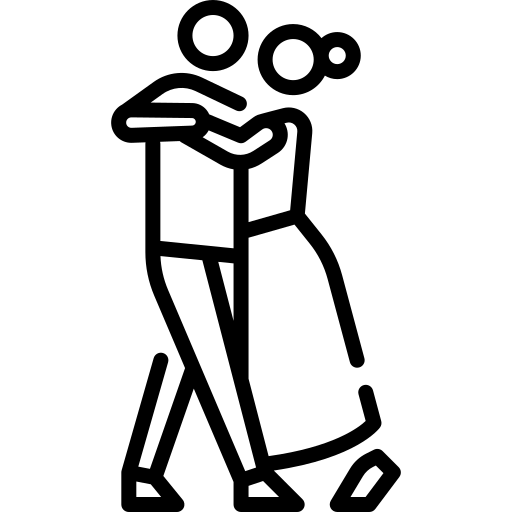
\includegraphics[width=0.0#1\textwidth]{icons/dancing.png}}

\newcommand{\iconratiotoc}{23}
\newcommand{\iconratiosec}{70}
\newcommand{\dparagraph}[1]{\vspace{0.25cm}\textbf{\Large#1}\par\vspace{0.05cm}}
\newcommand{\dsubparagraph}[1]{\textbf{\large #1}}

\newcommand{\loadIllustration}[3][1.0]{\begin{center}\includegraphics[width=#1\textwidth]{#2#3.png}\end{center}}
\newcommand{\loadSCDScheme}[2][1.0]{\loadIllustration[#1]{SCDschemes/}{#2}}


\newcommand{\Interdance}[1]{\section[#1]{\LARGE #1}\;\par}
\newcommand{\Dance}[5]{\newcommand{#1}{\section[\texorpdfstring{#2{\iconratiotoc}}{} #3]{#2{\iconratiosec} \LARGE #4}\large{\;\par #5}\par}}
\newcommand{\DanceSmall}[5]{\newcommand{#1}{\begin{minipage}{\textwidth}\section[\texorpdfstring{#2{\iconratiotoc}}{} #3]{#2{\iconratiosec} \LARGE #4}\large{\;\par #5}\end{minipage}\par}}


\newcommand{\SCDance}[4]{\DanceSmall{#1}{\SCD}{SCD #2}{Шотландский контрданс}{
\vspace{0.25cm}
\loadIllustration[1.0]{SCDschemes/}{#3}
#4
}}

\newcommand{\microparagraph}[1]{\vspace{0.1cm}\textbf{\Large $\blacktriangleright$ #1}\par}
\newcommand{\textScheme}{Схема танца:}
\newcommand{\Scheme}{\microparagraph{\textScheme}}
\newcommand{\Start}{\microparagraph{Исходное положение:}}
\newcommand{\Note}[1]{\begin{minipage}{\textwidth}\microparagraph{Примечание:} #1 \end{minipage}}
\newcommand{\Variation}[1]{\begin{minipage}{\textwidth}\microparagraph{Варианты исполнения:} #1 \end{minipage}}
\newcommand{\Reminder}[2]{\begin{minipage}{\textwidth}\addtocontents{toc}{\protect\contentsline{section}{#1}{$\square$}{}}\vspace{0.1cm}{\huge\textbf{#1}}\;\par\vspace{0.1cm}#2\end{minipage}}
%\newcommand{\Interdance}[2][$\square$]{\addtocontents{toc}{\protect\contentsline{section}{#2}{$\square$}{}}\vspace{0.1cm}\par#1\qquad {\huge\textbf{#2}}\;\par}

% \newcommand{\Dchapter}[1]{}
\newcommand{\Dchapter}[1]{\addtocontents{toc}{\protect\contentsline{section}{#1\dotfill}{\dots}{}}\vspace{0.1cm}\par {\Huge\textbf{#1}}\;\par}
\newcommand{\dtable}[3]{
\begin{tabular}
  {>{\raggedleft\arraybackslash}p{#1\textwidth}
   >{\raggedright\arraybackslash}p{#2\textwidth}
  }
  #3
\end{tabular}
}
\newcommand{\DanceTable}[4]{
\begin{minipage}{\textwidth}
\dparagraph{#1}
\dtable{#3}{#4}{#2}
\end{minipage}
}

\ifthenelse{\isundefined{\mobile}}{
\newcommand{\sepa}{0.07}
\newcommand{\sepb}{0.93}
\newcommand{\sepc}{0.1}
\newcommand{\sepd}{0.9}
}{
\newcommand{\sepa}{0.1}
\newcommand{\sepb}{0.90}
\newcommand{\sepc}{0.15}
\newcommand{\sepd}{0.85}
}

\newcommand{\StandartTable}[1]{\dtable{\sepa}{\sepb}{#1}}
\newcommand{\DancePart}[2]{\DanceTable{#1}{#2}{\sepa}{\sepb}}
\newcommand{\DanceBeat}[2]{\DanceTable{#1}{#2}{\sepc}{\sepd}}
\newcommand{\DanceBeatNCap}[1]{
\begin{minipage}{\textwidth}
\dtable{\sepc}{\sepd}{#1}
\end{minipage}
}
\newcommand{\DanceScheme}[1]{\DancePart{\textbf{\Large $\blacktriangleright$ \textScheme}}{#1}}